\documentclass[a4paper,12pt]{article}
\usepackage[utf8]{inputenc}
\usepackage[spanish]{babel}
\usepackage{color}
\usepackage{parskip}
\usepackage{graphicx}
\usepackage{multirow}
\usepackage{listings}
\usepackage{vmargin}
\usepackage{datetime}
\newdate{date}{2}{11}{2017}
\graphicspath{ {imagenes/} }
\definecolor{mygreen}{rgb}{0,0.6,0}
\definecolor{lbcolor}{rgb}{0.9,0.9,0.9}
\usepackage{epstopdf}
\usepackage{float}


\setpapersize{A4}
\setmargins{2.5cm}       % margen izquierdo
{1.5cm}                        % margen superior
{16.5cm}                      % anchura del texto
{23.42cm}                    % altura del texto
{10pt}                           % altura de los encabezados
{1cm}                           % espacio entre el texto y los encabezados
{0pt}                             % altura del pie de página
{2cm}     

\lstset{
    tabsize=4,    
%   rulecolor=,
    language=[GNU]C++,
        basicstyle=\tiny,
        aboveskip={1.5\baselineskip},
        columns=fixed,
        showstringspaces=false,
        extendedchars=false,
        breaklines=true,
        prebreak = \raisebox{0ex}[0ex][0ex]{\ensuremath{\hookleftarrow}},
        frame=single,
        showtabs=false,
        showspaces=false,
        showstringspaces=false,
        identifierstyle=\ttfamily,
        keywordstyle=\color[rgb]{0,0,1},
        commentstyle=\color[rgb]{0.026,0.112,0.095},
        stringstyle=\color{red},
        numberstyle=\color[rgb]{0.205, 0.142, 0.73},
%        \lstdefinestyle{C++}{language=C++,style=numbers}’.
}


\begin{document}
\title{Práctica de Laboratorio 3}
\author{
Christofer Fabián Chávez Carazas \\
\small{Universidad Nacional de San Agustín de Arequipa} \\
\small{Escuela Profesional de Ciencia de la Computación} \\
\small{Computación Gráfica}
}
\date{\displaydate{date}}

\maketitle

\begin{enumerate}
 \item \textbf{Compile y ejecute el siguiente código}
 
 \textbf{Resultados:}
 \begin{figure}[H]
  \centering
  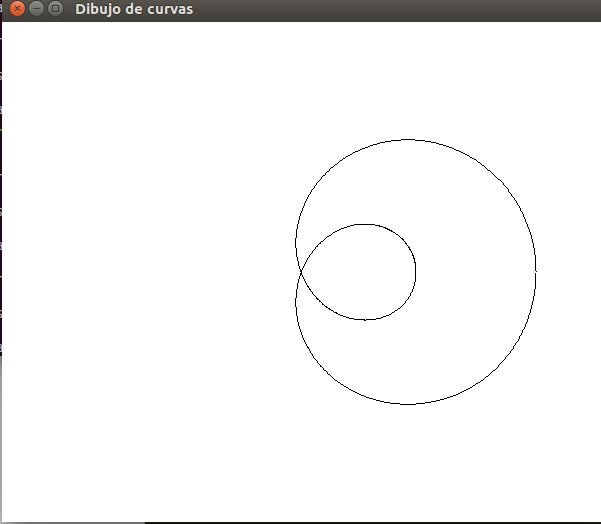
\includegraphics[scale = 0.3]{1.png}
 \end{figure}
 \begin{figure}[H]
  \centering
  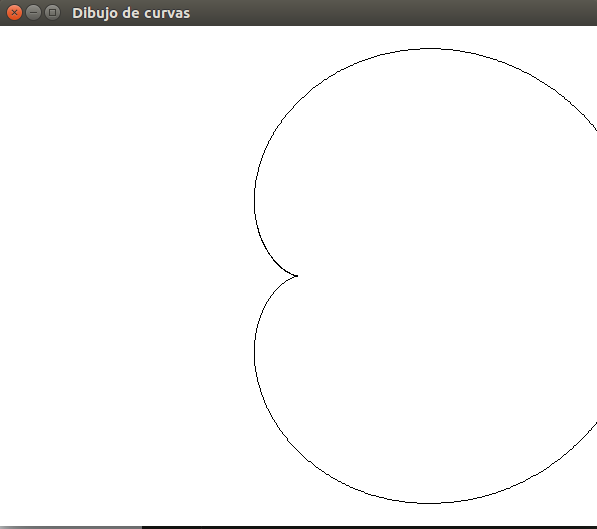
\includegraphics[scale = 0.3]{2.png}
 \end{figure}
 \begin{figure}[H]
  \centering
  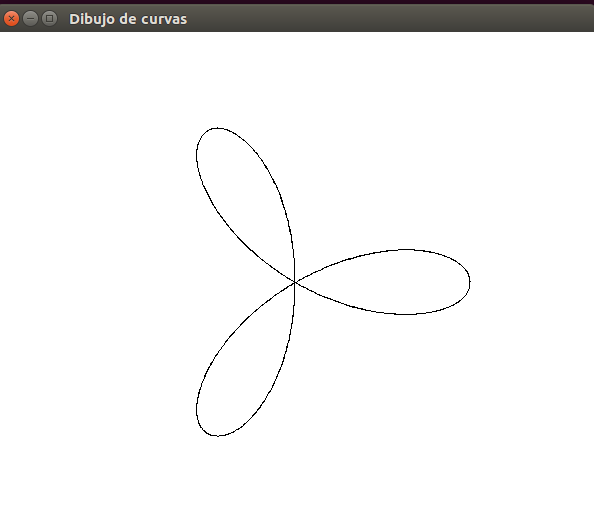
\includegraphics[scale = 0.3]{3.png}
 \end{figure}
 \begin{figure}[H]
  \centering
  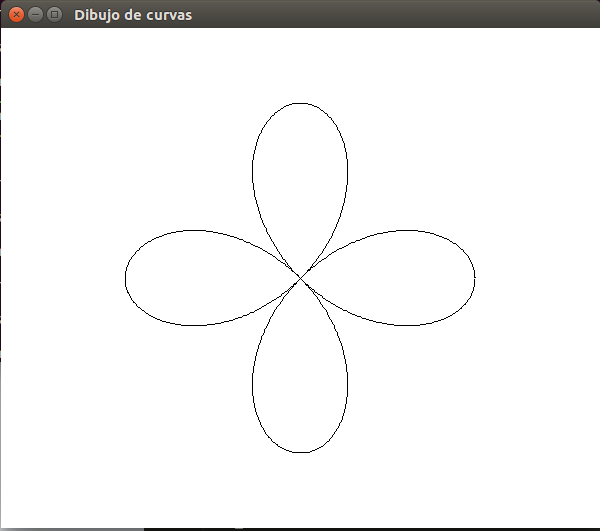
\includegraphics[scale = 0.3]{4.png}
 \end{figure}
 \begin{figure}[H]
  \centering
  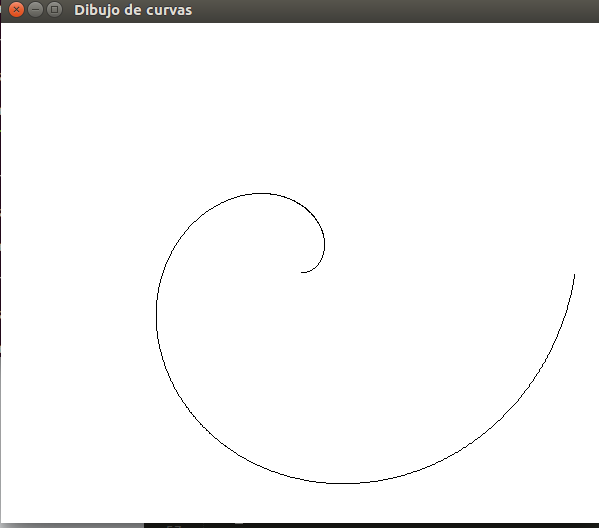
\includegraphics[scale = 0.3]{5.png}
 \end{figure}

 \item \textbf{Implique que función cumple cada línea de código:}
 
 Lo primero que hace el programa es pedirnos qué tipo de curva va a dibujar. Esto lo hace en la siguiente función:
 
 \begin{lstlisting}
void displayFcn(void){
    GLint curveNum;
    glClear(GL_COLOR_BUFFER_BIT);
    cout<<"\nIngrese el entero correspondiente a\n";
    cout<<"una de las siguientes cuevas.\n";
    cout<<"Presione otra tecla para salir.\n";
    cout<<"\n1-caracola, 2-cardioide, 3-trebol(3 hojas), 4-trebol(4 hojas), 5-espiral: ";
    cin>>curveNum;

    if(curveNum == 1 or curveNum == 2 or curveNum == 3 or curveNum == 4 or curveNum == 5){
        drawCurve(curveNum);
    }
    else exit(0);
    glFlush();
}
 \end{lstlisting}

 La función principal del programa es \textit{drawCurve}.
 
 \begin{lstlisting}
    const GLint a = 175, b = 60;

    GLfloat r, theta, dtheta = 1.0 / float(a);
    GLint x0 = 300, y0 = 250;
 \end{lstlisting}
 
 Las variables \textit{a} y \textit{b} son el ancho y el largo que va a tener la cueva. La variable \textit{dtheta} es el desplazamiento de \textit{theta}.
 Las variables \textit{x0} y \textit{y0} son las coordenadas del punto central de la curva.
 
 \begin{lstlisting}
    curvePt[0].x = x0;
    curvePt[0].y = y0;

    switch(curveNum){
        case limacon:
            curvePt[0].x += a + b; break;
        case cardioid:
            curvePt[0].x += a + a; break;
        case threeLeaf:
            curvePt[0].x += a; break;
        case fourLeaf:
            curvePt[0].x += a; break;
        case spiral:
            break;
        default:
            break;
    }
 \end{lstlisting}
 
 En esta parte del código se inicializa el punto donde comenzará a dibujarse la curva, y esto se hace dependiendo de la curva que queramos dibujar.
 
 \begin{lstlisting}
    theta = dtheta;
    while(theta < twoPI){
        switch(curveNum){
            case limacon:
                r = a * cos(theta) + b; break;
            case cardioid:
                r = a * (1 + cos(theta)); break;
            case threeLeaf:
                r = a * cos(3 * theta); break;
            case fourLeaf:
                r = a * cos(2 * theta); break;
            case spiral:
                r = (a / 4.0) * theta; break;
            default:
                break;
        }

        curvePt[1].x = x0 + r * cos(theta);
        curvePt[1].y = y0 + r * sin(theta);
        lineSegment(curvePt[0], curvePt[1]);

        curvePt[0].x = curvePt[1].x;
        curvePt[0].y = curvePt[1].y;
        theta += dtheta;
    }
 \end{lstlisting}

  En esta parte del código se halla el radio, según la curva que queramos dibujar, para poder hallar el siguiente punto de la curva. Luego, se dibuja una linea desde el
  punto actual hasta el punto recién hallado. Después, el punto actual se vuelve el punto recién hallado y se suma a \textit{theta} el desplazamiento para la siguiente iteración.
  
  
 \item \textbf{Implemente el algoritmo DDA para el trazado de líneas}
 
 \begin{lstlisting}
#include <GL/glut.h>
#include <iostream>
#include <cmath>


GLsizei winWidth = 600, winHeight = 500;

struct Point{
    GLint x;
    GLint y;
};

void init(void){
    glClearColor(1.0, 1.0, 1.0, 1.0);
    glMatrixMode(GL_PROJECTION);
    gluOrtho2D(0.0, 600.0, 0.0, 500.0);
}

void drawPoint(Point p){
    glBegin(GL_POINTS);
        glVertex2i(p.x, p.y);
    glEnd();
}

void drawLine(Point a, Point b){
    glBegin(GL_LINES);
        glVertex2i(a.x, a.y);
        glVertex2i(b.x, b.y);
    glEnd();
}

void DDA(Point ini, Point final){
    GLint deltaX = final.x - ini.x;
    GLint deltaY = final.y - ini.y;
    GLint pasos = -1;
    GLint incrementoX = -1;
    GLint incrementoY = -1;
    Point actual;
    if(abs(deltaX) > abs(deltaY)) pasos = abs(deltaX);
    else pasos = abs(deltaY);
    incrementoX = deltaX / pasos;
    incrementoY = deltaY / pasos;
    actual.x = ini.x;
    actual.y = ini.y;
    drawPoint(actual);
    for(int i = 0; i < pasos; i++){
        actual.x += incrementoX;
        actual.y += incrementoY;
        drawPoint(actual);
    }
}

void display(){
    Point a;
    Point b;
    a.x = 50;
    a.y = 50;
    b.x = 400;
    b.y = 400;
    glClear(GL_COLOR_BUFFER_BIT);
    glColor3f(1.0, 0.0, 0.0);
    DDA(a,b);
    glFlush();

}


int main(int argc, char **argv){
    glutInit(&argc, argv);
    glutInitDisplayMode(GLUT_SINGLE | GLUT_RGB);
    glutInitWindowPosition(100,100);
    glutInitWindowSize(winWidth, winHeight);
    glutCreateWindow("Dibujo de curvas");

    init();
    glutDisplayFunc(display);


    glutMainLoop();

}
 \end{lstlisting}
 
 \begin{figure}[H]
  \centering
  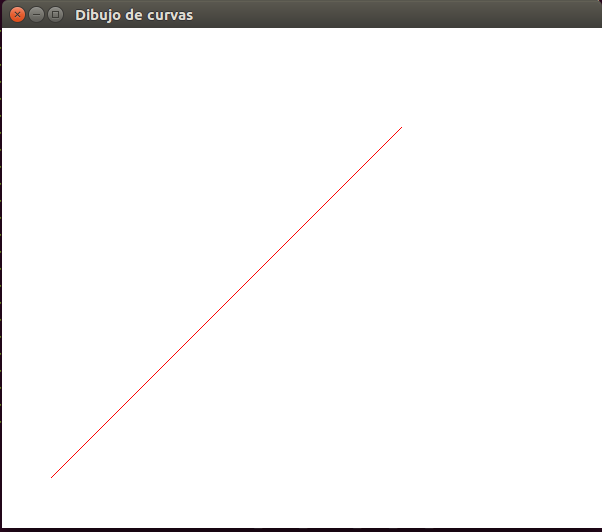
\includegraphics[scale = 0.3]{6.png}
  \caption{Resultados}
 \end{figure}

 \item \textbf{Implemente el algoritmo Bresenham para el trazado de líneas}
 
 \begin{lstlisting}
#include <GL/glut.h>
#include <iostream>
#include <cmath>
#include <algorithm>

using namespace std;

GLsizei winWidth = 600, winHeight = 500;

struct Point{
    GLint x;
    GLint y;
};

void init(void){
    glClearColor(1.0, 1.0, 1.0, 1.0);
    glMatrixMode(GL_PROJECTION);
    gluOrtho2D(0.0, 600.0, 0.0, 500.0);
}

void drawPoint(Point p){
    glBegin(GL_POINTS);
        glVertex2i(p.x, p.y);
    glEnd();
}

void drawLine(Point a, Point b){
    glBegin(GL_LINES);
        glVertex2i(a.x, a.y);
        glVertex2i(b.x, b.y);
    glEnd();
}

void bresenham(Point ini, Point fin){
    GLint dX = fin.x - ini.x;
    GLint dY = fin.y - ini.y;
    GLint IncYi;
    GLint IncXi;
    GLint IncXr;
    GLint IncYr;
    GLint avR;
    GLint av;
    GLint avI;
    if(dY >= 0) IncYi = 1;
    else{
        dY = -dY;
        IncYi = -1;
    }
    if(dX >= 0) IncXi = 1;
    else{
        dX = -dX;
        IncXi = -1;
    }
    if(dX >= dY){
        IncYr = 0;
        IncXr = IncXi;
    }
    else{
        IncXr = 0;
        IncYr = IncYi;
        swap(dX,dY);
    }
    Point actual;
    actual.x = ini.x;
    actual.y = ini.y;
    avR = 2 * dY;
    av = avR - dX;
    avI = av - dX;
    while(actual.x != fin.x){
        drawPoint(actual);
        if(av >= 0){
            actual.x += IncXi;
            actual.y += IncYi;
            av += avI;
        }
        else{
            actual.x += IncXr;
            actual.y += IncYr;
            av += avR;
        }
    }
}



void display(){
    Point a;
    Point b;
    a.x = 50;
    a.y = 400;
    b.x = 400;
    b.y = 50;
    glClear(GL_COLOR_BUFFER_BIT);
    glColor3f(1.0, 0.0, 0.0);
    bresenham(a,b);
    glFlush();

}


int main(int argc, char **argv){
    glutInit(&argc, argv);
    glutInitDisplayMode(GLUT_SINGLE | GLUT_RGB);
    glutInitWindowPosition(100,100);
    glutInitWindowSize(winWidth, winHeight);
    glutCreateWindow("Dibujo de curvas");

    init();
    glutDisplayFunc(display);


    glutMainLoop();

}
 \end{lstlisting}
 
 \begin{figure}[H]
  \centering
  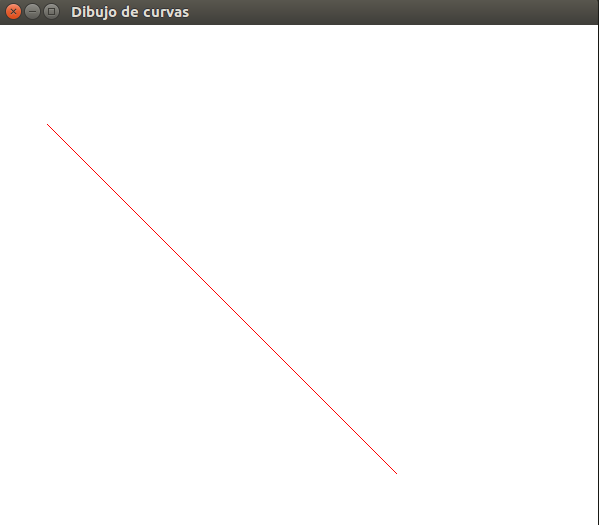
\includegraphics[scale = 0.3]{7.png}
  \caption{Resultados}
 \end{figure}

 \item \textbf{Implemente el algoritmo del punto medio para la generación de círculos}

 \begin{lstlisting}
#include <GL/glut.h>
#include <iostream>
#include <cmath>
#include <algorithm>

using namespace std;

GLsizei winWidth = 600, winHeight = 500;

struct Point{
    GLint x;
    GLint y;
};

void init(void){
    glClearColor(1.0, 1.0, 1.0, 1.0);
    glMatrixMode(GL_PROJECTION);
    gluOrtho2D(0.0, 600.0, 0.0, 500.0);
}

void setPixel(GLint x, GLint y){
    glBegin(GL_POINTS);
        glVertex2i(x,y);
    glEnd();
}


void circlePlotPoints(Point circCtr, Point circPt){
    setPixel(circCtr.x + circPt.x,circCtr.y + circPt.y);
    setPixel(circCtr.x - circPt.x,circCtr.y + circPt.y);
    setPixel(circCtr.x + circPt.x,circCtr.y - circPt.y);
    setPixel(circCtr.x - circPt.x,circCtr.y - circPt.y);
    setPixel(circCtr.x + circPt.y,circCtr.y + circPt.x);
    setPixel(circCtr.x - circPt.y,circCtr.y + circPt.x);
    setPixel(circCtr.x + circPt.y,circCtr.y - circPt.x);
    setPixel(circCtr.x - circPt.y,circCtr.y - circPt.x);
}

void circleMidPoint(Point circCtr, GLint radius){
    Point circPt;
    GLint p = 1 - radius;
    circPt.x = 0;
    circPt.y = radius;
    circlePlotPoints(circCtr, circPt);
    while(circPt.x < circPt.y){
        circPt.x++;
        if(p < 0) p += 2 * circPt.x + 1;
        else{
            circPt.y--;
            p += 2 * (circPt.x - circPt.y) + 1;
        }
        circlePlotPoints(circCtr, circPt);
    }
}

void display(){
    Point center;
    center.x = 300;
    center.y = 250;
    glClear(GL_COLOR_BUFFER_BIT);
    glColor3f(1.0, 0.0, 0.0);
    circleMidPoint(center, 100);
    glFlush();
}

int main(int argc, char **argv){
    glutInit(&argc, argv);
    glutInitDisplayMode(GLUT_SINGLE | GLUT_RGB);
    glutInitWindowPosition(100,100);
    glutInitWindowSize(winWidth, winHeight);
    glutCreateWindow("Mid Point");

    init();
    glutDisplayFunc(display);


    glutMainLoop();

}
 \end{lstlisting}

 
 \begin{figure}[H]
  \centering
  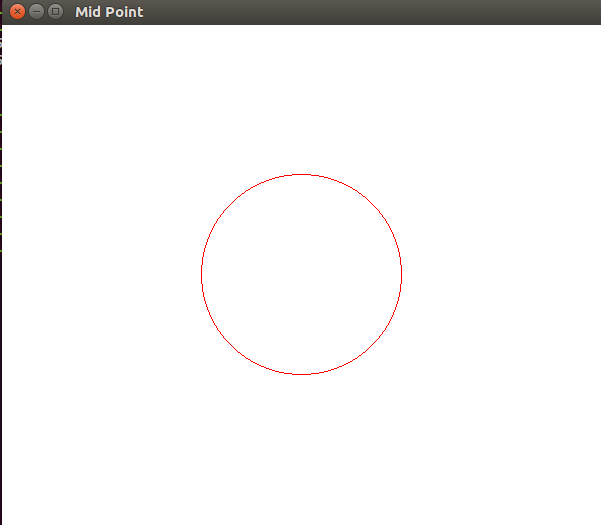
\includegraphics[scale = 0.3]{8.png}
 \end{figure}

 \item \textbf{Implementar el algoritmo del punto medio para la generación de elipses}
 
 \begin{lstlisting}
#include <GL/glut.h>
#include <iostream>
#include <cmath>
#include <algorithm>

using namespace std;

GLsizei winWidth = 600, winHeight = 500;

struct Point{
    GLint x;
    GLint y;
};

void init(void){
    glClearColor(1.0, 1.0, 1.0, 1.0);
    glMatrixMode(GL_PROJECTION);
    gluOrtho2D(0.0, 600.0, 0.0, 500.0);
}

void setPixel(GLint x, GLint y){
    glBegin(GL_POINTS);
        glVertex2i(x,y);
    glEnd();
}

void elipcePlotPoints(Point centro, Point actual){
    setPixel(centro.x + actual.x, centro.y + actual.y);
    setPixel(centro.x - actual.x, centro.y + actual.y);
    setPixel(centro.x + actual.x, centro.y - actual.y);
    setPixel(centro.x - actual.x, centro.y - actual.y);
}

void elipceMidPoint(Point centro, GLint radiusX, GLint radiusY){
    GLdouble p1, p2;
    GLint rX2, rY2;
    Point actual;
    actual.x = 0;
    actual.y = radiusY;
    rX2 = pow(radiusX,2);
    rY2 = pow(radiusY,2);
    p1 = rY2 - (rX2 * radiusY) + (0.25 * rX2);
    while((rY2 * actual.x) < (rX2 * actual.y)){
        actual.x++;
        if(p1 < 0) p1 += (2 * rY2 * actual.x) + rY2;
        else{
            actual.y--;
            p1 += (2 * rY2 * actual.x) - (2 * rX2 * actual.y) + rY2;
        }
        elipcePlotPoints(centro,actual);
    }
    p2 = (rY2) * pow((actual.x + 0.5), 2) + (rX2) * pow((actual.y - 1), 2) - (rX2 * rY2);
    while(actual.y > 0){
        actual.y--;
        if(p2 > 0) p2 -= (2 * rX2 * actual.y) + rX2;
        else{
            actual.x++;
            p2 += (2 * rY2 * actual.x) - (2 * rX2 * actual.y) + rX2;
        }
        elipcePlotPoints(centro,actual);
    }
}

void display(){
    Point center;
    center.x = 300;
    center.y = 250;
    glClear(GL_COLOR_BUFFER_BIT);
    glColor3f(1.0, 0.0, 0.0);
    elipceMidPoint(center, 50, 200);
    elipceMidPoint(center, 200, 50);

    glFlush();
}

int main(int argc, char **argv){
    glutInit(&argc, argv);
    glutInitDisplayMode(GLUT_SINGLE | GLUT_RGB);
    glutInitWindowPosition(100,100);
    glutInitWindowSize(winWidth, winHeight);
    glutCreateWindow("Mid Point");

    init();
    glutDisplayFunc(display);


    glutMainLoop();

}

 \end{lstlisting}

  \begin{figure}[H]
   \centering
   
\includegraphics[scale = 0.3]{9.png}
   \caption{Resultados}
  \end{figure}

 \item \textbf{Realice un diseño artístico (Dibujo) con los algoritmos implementados en 3,4,5 y 6}
 
 Función que utiliza los anteriores algoritmos para dibujar arte.
 
 \begin{lstlisting}
void arte(){
	Point rec1;
	Point rec2;
	Point rec3;
	Point rec4;
	Point centro;
	centro.x = winWidth / 2;
	centro.y = winHeight / 2;
	GLint desplRec = 5;
	GLint finalRec = 50;
	glClear(GL_COLOR_BUFFER_BIT);
    glColor3f(1.0, 0.0, 0.0);
    for(GLint i = desplRec; i < finalRec; i += desplRec){
    	rec1.x = i; rec1.y = i;
    	rec2.x = i; rec2.y = winHeight - i;
    	rec3.x = winWidth - i; rec3.y = winHeight - i;
    	rec4.x = winWidth - i; rec4.y = i;	
    	DDA(rec1, rec2);
		bresenham(rec2, rec3);
		DDA(rec3, rec4);
		bresenham(rec1, rec4);
    }
    GLint desplCirc = 5;
    GLint finalCirc = 50;
    GLint desplXElip = 5;
    GLint desplYElip = 1;
    GLint finalElip = 50;
    centro.x -= 200;
    for(int k = 0; k < 5; k++){
    	circleMidPoint(centro, 1);
    	for(GLint i = desplCirc; i < finalCirc; i += desplCirc){
    		circleMidPoint(centro, i);
    	}
    	centro.x += 100;
    }
    
    centro.x = winWidth / 2;
    centro.y -= 100;
    GLint rX = 1;
    GLint rY = 2;
    while(rX != finalElip and rY != finalElip){
    	elipceMidPoint(centro, rX, rY);
    	rX += desplXElip;
    	rY += desplYElip;
    }
    rX -= desplXElip;
    rY -= desplYElip;
    centro.y += 200;
    elipceMidPoint(centro, rX, rY);
    circleMidPoint(centro, rY);

    for(int i = rY / 2; i != 5; i--){
    	circleMidPoint(centro, i);	
    }
	glFlush();
}
 \end{lstlisting}
 
 \begin{figure}[H]
  \centering
  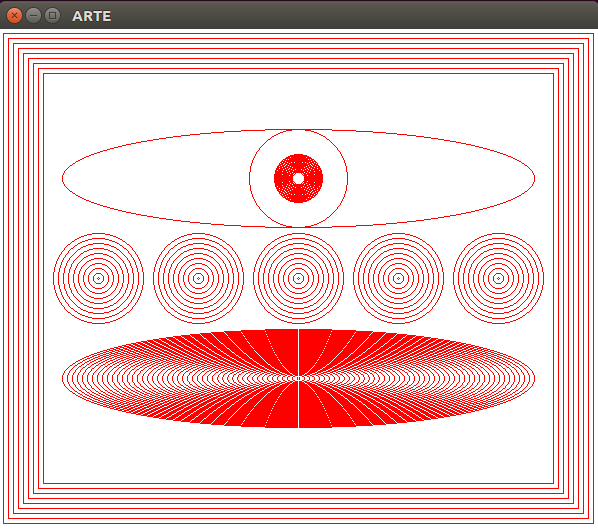
\includegraphics[scale = 0.5]{10.png}
  \caption{Resultados}
 \end{figure}


 
\end{enumerate}



\end{document}

